\section{OAuth2}
\label{auth:oauth2}

OAuth2 ist ein Standardprotokoll für die Benutzerautorisierung \cite{rfc6749}. \\ 

Der Autorisierungsserver des IdM-Providers muss gemäß RFC 6749 folgende \textit{Endpoints} bereitstellen:

\begin{table}[htb]
    \begin{tabularx}{\textwidth}{|c|X|}
        \hline
\textbf{Endpoint} & \textbf{Funktion} \\ \hline
Authorization & Initiierung der Autorisierung und Benutzerzustimmung durch parametrisierten Aufruf \\ \hline
Token & Liefert gegen Authorization Code Access Token zurück \\ \hline
    \end{tabularx}

        \caption{Endpunkte, die durch den IdM-Provider für die Anmeldung per OAuth2 zur Verfügung gestellt werden müssen}
        \label{tab:auth:endpoints}
\end{table}

OAuth2 definiert sogenannte \textit{Grant Types}, die vom \textit{Client} über das Setzen eines oder mehrerer \textit{response$\_$type} beim Aufruf des \textit{Authorization Endpoint} gewählt werden können. 
Diese \textit{Grant Types} beschreiben Möglichkeiten, wie ein Client einen \textit{Access Token} erlangt, über den im Namen des Benutzers anschließend eine API aufgerufen werden kann. 
Während \textit{response$\_$type=code} den \textit{Authorization Code Grant} initiiert, liefert \textit{response$\_$type=token} den Access Token direkt nach Autorisierung zurück. 
Zudem lassen sich über \textit{Access Token Scopes} vom Client Anwendungsbereiche des vom Autorisierungsserver gelieferten Access Tokens anfordern \cite[Abschnitt~3.3]{rfc6749}. \\

Die \textit{Internet Engineering Task Force (IETF)} empfiehlt die Verwendung des \textit{Authorization Code Grant} \cite[Unterabschnitt~2.1.1]{ietf-oauth-security-topics-18}. 
Je nachdem, ob es sich um einen \textit{Confidential} oder \textit{Public Client} handelt, d.h., ob ein \textit{Client Secret} verwendet werden kann, wird ein \textit{Proof Key for Code Exchange (PKCE)} empfohlen bzw. vorgeschrieben. 
Der PKCE ist eine Erweiterung des \textit{Authorization Code Grant}, um Cross-Site-Request-Forgery (CSRF) oder Authentication-Code-Injection-Angriffe zu verhindern \cite{rfc7636}. \\

Der Ablauf der Autorisierung per OAuth2-Protokoll im \textit{Authorization Code Grant} ist in Abbildung \refabb{fig:auth-code-grant} dargestellt. 
Dieser wird durch den \textit{Client} gestartet, gefolgt von der Autorisierung durch den \textit{Resource Owners} beim Autorisierungserver. 
Der Autorisierungserver sendet einen \textit{Authorization Code} an den \textit{Client}, der diesen wiederum direkt beim Autorisierungsserver gegen den \textit{Access Token} tauscht. Über den Access Token erhält der Benutzer schließlich Zugriff auf die REST-API.

\begin{figure}[htbp]
\centering
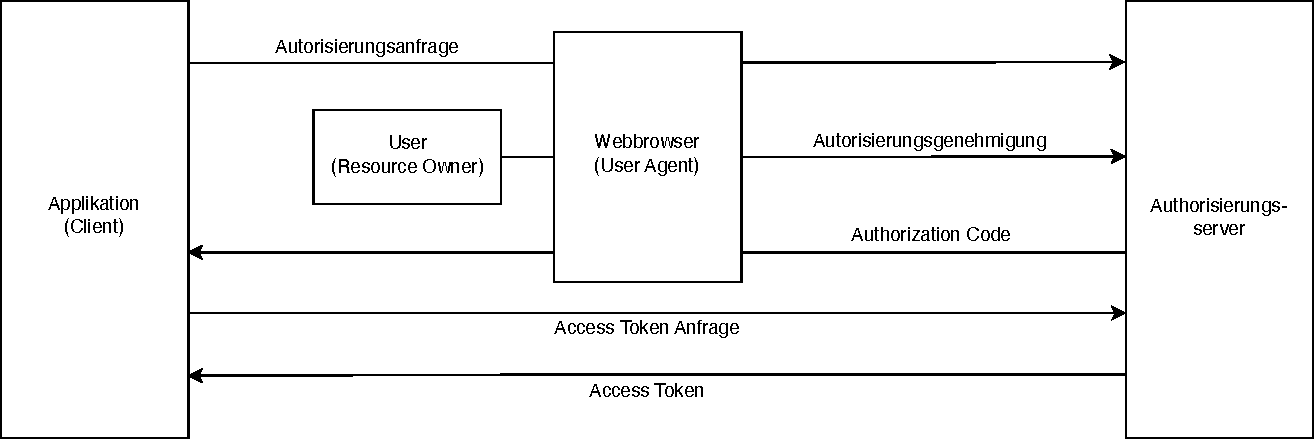
\includegraphics[width=\textwidth]{Authentication_Code_Grant.pdf}
\caption{Ablauf des Authentication Code Grant}
\label{fig:auth-code-grant}
\end{figure}
